\documentclass{article}
%\documentclass[aps, twocolumn, tightenlines,amscd,amsmath,amssymb,verbatim]{revtex4}
\usepackage{latexsym}
\usepackage{amssymb,amsmath}
\usepackage{custom2}
\usepackage{graphicx} % for figures
\usepackage{epstopdf} % so can use EPS or PDF figures
%\usepackage{subfig}
\usepackage{caption}
\usepackage{subcaption}
\usepackage{url}
\usepackage{amssymb,amsfonts}
\usepackage[all,arc]{xy}
\usepackage{enumerate}
\usepackage{mathrsfs}
\usepackage{booktabs}
\usepackage[pdftex]{hyperref}
\usepackage{lscape}
\captionsetup{justification=RaggedRight, singlelinecheck=false}
\newcommand{\ra}[1]{\renewcommand{\arraystretch}{#1}}
\newcommand{\argmax}{\text{argmax}}
\newcommand{\Tr}{\text{Tr}}
%\newtheorem{claim}{Claim}

\addtolength{\evensidemargin}{-.5in}
\addtolength{\oddsidemargin}{-.5in}
\addtolength{\textwidth}{1.4in}
\addtolength{\textheight}{1.4in}
\addtolength{\topmargin}{-.5in}

\pagestyle{empty}

\begin{document}


\begin{center}
{\bf \LARGE{Information Gathering Strategies in Social Networks}}
\vspace{10pt}
\\ Eleanor Brush
\\ December 27, 2012
\end{center}

\tableofcontents


\section{The Model}

We consider a network where each agent has an interval variable, keeping track of, for example, direction or velocity of movement or a desired location, and uses the variables of the neighbors to whom it is connected to update its variable.  More concretely, there are $n$ nodes, which each have a variable $x_i$ and receive information from its neighbors weighted by a factor $w_{ij}$ such that $\sum_jw_{ij}=1$ for all $i=1,\dots,n$.  For instance, node $i$ may have $k$ connections, each of which it values equally so that $w_{ij}=1/k$ for those nodes from whom $i$ receives information and $w_{ij}=0$ otherwise.  In continuous time, the dynamics of the model are given by
$$\frac{d x_i}{dt}(t)=\sum_jw_{ij}(x_j(t)-x_i(t))+\xi_i$$ 
where $\xi_i$ is random noise.  Let $L$ be the Laplacian of the weighted matrix given by the $w_{ij}$ so that
$$L_{ij}=\left\{\begin{array}{cccc}
1& , & \text{ if } i=j \\
-w_{ij} & , & \text{ else}
\end{array}\right.$$
so that the model can be written as 
$$\dot{x}(t)=-Lx(t)+\xi$$

Suppose there is external or environmental information that the agents can gather and that the agents perform better if they gather more accurate information.  In particular, suppose that a node receives an external signal $s$, which the rest of the agents want to learn as quickly and as accurately as possible.  We will suppose that the agent that receives the external signal is chosen at random.  For now, we assume that the first node is chosen.   Having received the external signal, that agent no longer listens to the other agents in the system, so that its dynamics are changed to $x_1(t)=s$ for all $t$.   The dynamics for the other nodes become
$$\frac{dx_i}{dt}=w_{i1}(s-x_i(t))+\sum_{j\neq 1}w_{ij}(x_j(t)-x_i(t))+\xi_i(t).$$
A consensus state is again the equilibrium, but now the consensus value is fixed at $s$, the value of the external signal.  

%%%%%%%%%%%%%%
\section{Measures of deviation\label{deviations}}
Different nodes in the network might be subject to different sources and magnitudes of noise.  We will always assume that $\E[\xi_i]=0$.  Let $d_i=Var[\xi_i]$ and $D=diag(d_1,\dots,d_n)$.  In particular, we will set $d_i$ equal to the number of neighbors influencing node $i$, so that nodes with more neighbors make noisier estimates.

Let $y$ represent the distance between the vector of opinions and consensus, i.e.
$y=QxQ^T,$
where $Q\in\R^{n-1\times n}$ is such that $Q\vec{1}=0$ , $QQ^T=I_{n-1}$, and $Q^TQ=I_n-\frac{1}{n}\vec{1}\times\vec{1}^T$.   
Then 
\begin{equation}
\dot{y}(t)=-\overline{L}y(t)+Q\xi(t) \notag
\end{equation}
where $\overline{L}=QLQ^T$.  As shown in \cite{Young:2010fk}, if $\Sigma_y(t)=\E[y(t)y(t)^T]$,  $\Sigma_y$ at equilibrium solves
\begin{equation} 0=-\overline{L}\Sigma_y-\Sigma_y\overline{L}^T+D. \label{h2norm}
\end{equation}
If we instead consider deviation from the external signal, $\delta_i(t)=x_i(t)-s$,
\begin{align*}
\dot{\delta_i}(t)&=\dot{x_i}(t)
\\&=\sum_jw_{ij}(x_j(t)-x_i(t))+\xi_i(t)
\\&=\sum_jw_{ij}(\delta_j(t)-\delta_i(t))+\xi_i(t)
\\&=\sum_{j\neq 1}w_{ij}\delta_j(t)-\delta_i(t)\sum_jw_{ij}+\xi_i(t) \text{ since $\delta_1(t)\equiv 0$}
\\ \text{ so that }\dot{\delta}(t)&=-L^1\delta(t)+\xi(t)
\end{align*}
where $L^1$ is $L$ with the first row and column removed and $\delta(t)=(\delta_2(t)\dots\delta_n(t))$.
If $\Sigma(t)=\E[\delta(t)\delta(t)^T]$,  $\Sigma$ at equilibrium solves the analogous Lyapunov equation,
\begin{equation}
0=-L^1\Sigma-\Sigma(L^1)^T+D. \label{h2mod}
\end{equation}

\section{Relationship between consensus and external signal models}
\begin{claim} \label{myconjecture}
TO BE PROVED:  Let $L$ be the Laplacian of the weighted matrix and $L^1$ be $L$ without its first row and column.  Let the second smallest eigenvalue of $L$ be $\lambda$ and the smallest eigenvalue of $L^1$ be $\lambda_1$.  Then $1\geq \lambda \geq \lambda_1\geq 0$.  In particular,
\begin{enumerate}
\item $\lambda_1=0$ if and only if $w_{i1}=0$ for all $i$ and
\item if $w_{i1}=1$ for all $i$ then $\lambda_1=1$.
\end{enumerate}
\end{claim}

%Figure \ref{eigenvalue_comparison} shows that this is true for many randomly generated matrices.  
%\begin{figure}
%\begin{center}
%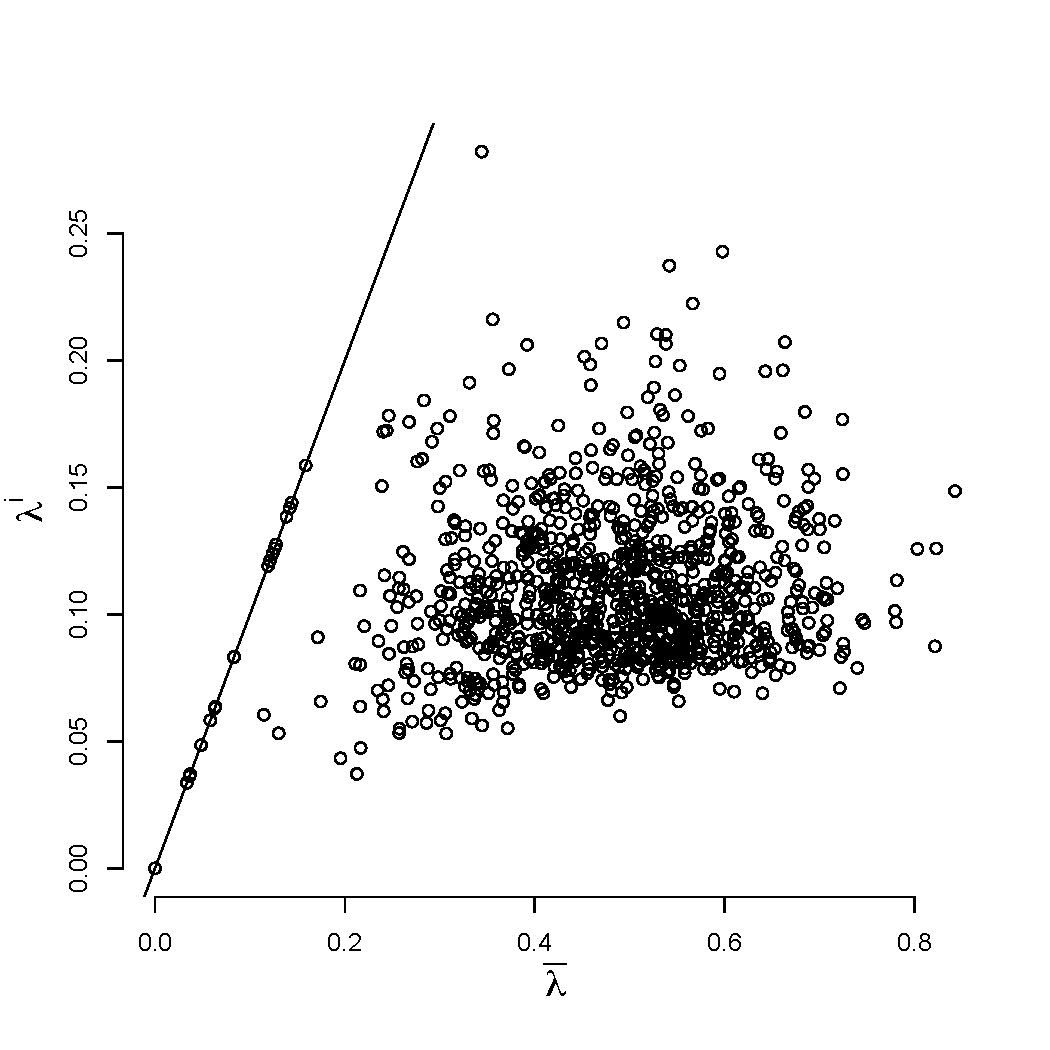
\includegraphics[width=.5\textwidth]{eigenvalue_comparison.pdf}
%\end{center}
%\caption{\label{eigenvalue_comparison} Here we plot the smallest eigenvalue $\lambda^i$ of the reduced Laplacian $L^i$ against the smallest eigenvalue $\overline{\lambda}$ of the transformed Laplacian $\overline{L}$, for several different matrices.  We find that $\lambda_i\leq \overline{\lambda}$.}
%\end{figure}

\begin{claim}
$||\delta(t)||\geq||y(t)||$ for all $t$.
\end{claim}

\begin{pf}
For the following, let $\langle x\rangle =\frac{\sum_ix_i}{n}$.
\begin{align*}
y&=x-\langle x\rangle \text{ and } \delta=x-s
\\ \Rightarrow ||y||^2&=\sum_i(x_i^2-2x_i\langle x\rangle+\langle x\rangle^2) \text{ and } ||\delta||^2=\sum_i(x_i^2-2x_is+s^2)
\\ \Rightarrow ||y||^2&=\sum_ix_i^2-2n\langle x\rangle^2+n\langle x\rangle^2 \text{ and } ||\delta||^2=\sum_ix_i^2-2ns\langle x\rangle+ns^2
\\ \Rightarrow ||\delta||^2-||y||^2&=ns^2-2ns\langle x\rangle+n\langle x\rangle^2
\\ &=n(\langle x\rangle-s)^2
\\ \Rightarrow ||\delta||^2-||y||^2&\geq 0 \text{ with equality iff } \langle x\rangle=s
\\ \Rightarrow ||\delta||^2&\geq||y||^2 \text{ with equality iff } \langle x\rangle=s
\\ \Rightarrow ||\delta||&\geq ||y|| \text{ with equality iff } \langle x\rangle=s
\end{align*}

\end{pf}

Therefore, $\lim_{t\to\infty}E[||\delta(t)||]\geq\lim_{t\to\infty}E[||y(t)||]$.

\section{Measures of Performance }

There are two general measures of performance: the speed with which the external signal can be learned and the steady state variance around the signal.  There is a tradeoff between these two measures.  As above let $L$ be the graph Laplacian of the network, $\overline{L}$ be the transformation of $L$, and $L^i$ be $L$ with the $i^{th}$ row and column removed, which describes how  a signal from individual $i$ propagates across the network.  Let $\lambda$ be the smallest eigenvalue of $\overline{L}$ and let $\lambda^i$ be the smallest eigenvalue of $L^i$ and $v^i$ its associated eigenvector.  Let $\Sigma_y$ and $\Sigma$ be the solutions to (\ref{h2norm}) and (\ref{h2mod}) respectively.  The eigenvalues $\lambda$ and $\lambda^i$ reflect how quickly consensus is reached or the external signal is learned and $\Sigma_y$ and $\Sigma$ are informative about the variance around consensus or the external signal.   We introduce a parameter $\alpha$ to represent the tradeoff between speed and variance.  

Our measure of group performance will be 
\begin{equation}
p_G=\left(\frac{1}{e^{-\lambda}}\right)^{(1-\alpha)}\left(\frac{\sqrt{N}}{\sqrt{\Tr(\Sigma_y)}}\right)^\alpha  \label{groupperf}
\end{equation}
where we take reciprocals so that a higher value of $p_G$ is associated with better performance (or fitness).  Our measure of individual performance for node $j$ will be 
\begin{equation}
p_j=\left(\frac{1}{e^{-\lambda^i}v_j}\right)^{(1-\alpha)}\left(\frac{1}{\sqrt{\Sigma_{jj}}}\right)^\alpha  \label{indperf}
\end{equation}



\section{Measure of a Node's Position Predicts Individual Performance }


\section{Equilibrium Strategies}

\subsection{Group Optimization }

If we assume the whole group has the same strategy, we can ask what strategy gives the best performance for the group (and for every individual, since they are assumed to be identical and thus receive the same payoffs), for various levels of the tradeoff $\alpha$ between speed and variance (Figure \ref{group_performance}).  Unsurprisingly, when speed is more important (low $\alpha$), it is best for the group for every node to have many neighbors.  When variance is more important (high $\alpha$), it is best for every node to have few neighbors.  What is somewhat surprising is that at intermediate levels of tradeoff, there is not a optimum intermediate between low and high strategies.  Instead, the landscape is rather flat and every strategy performs about equally well.

\begin{figure}
\begin{subfigure}{\textwidth}
\begin{center}
\includegraphics[width=\textwidth]{group_performance.eps}
\end{center}
\caption{$N=20$}
\end{subfigure}
\begin{subfigure}{\textwidth}
\begin{center}
\includegraphics[width=\textwidth]{group_performance_v2.eps}
\end{center}
\caption{$N=40$}
\end{subfigure}
\caption{\label{group_performance} This figure shows how group performance depends on strategy and tradeoff, assuming the whole group adopts the same strategy.  When speed is more important than variance (low $\alpha$), it is best for the group to be highly connected.  When variance is more important (high $\alpha$), it is best for the group to be less well connected.}
\end{figure}

\subsection{Individual Optimization }

\subsubsection{Adaptive Dynamics }

As shown in \cite{Nowak:2006uq}, if $f_i$ is the fitness of an invader and $g_i$ is the fitness of a resident when there are $i$ invaders, the probability of the number of invaders increasing by one is given by 
\begin{equation}
p_{i\to i+1}=\frac{i(N-i) f_i}{N(if_i+(N-i)g_i)}\label{probup}
 \end{equation}
and the probability of the number of invaders decreasing by one is given by 
\begin{equation}
p_{i\to i-1}=\frac{i(N-i) g_i}{N(if_i+(N-i)g_i)}\label{probdown}
 \end{equation}
 Together these give the probability that the invader will come to fixation in the population:
 \begin{equation}
 p_f=\frac{1}{1+\sum_{k=1}^{N-1}\Pi_{j=1}^k\frac{p_{i\to i+1}}{p_{i\to i-1}}} \label{probfix}
 \end{equation}
Here, individual fitnesses are given by (\ref{indperf}).  Since individual fitness depends on where the node is in the network in addition to its strategy, we say that $f_i=\langle p_j\rangle_{j: \text{ $j$ is an invader} }$ and $g_i=\langle p_j\rangle_{j: \text{ $j$ is an resident} }$ when there are $i$ invaders.   For an intermediate level of tradeoff between speed and variance, invaders with intermediate strategies have the highest probability of reaching fixation (Figure \ref{fixation_prob}).
 
 \begin{figure}
\begin{center}
\includegraphics[width=.75\textwidth]{fixation_prob.eps}
\end{center}
\caption{ \label{fixation_prob} This figure shows, for each pair of resident and invader strategies, the difference between the probability of the invader strategy reaching fixation and the fixation probability under neutral dynamics, $p_f-\frac{1}{N}$.  }
\end{figure}
 
 
A reasonable definition of an equilibrium is a situation in which, for a given pair of resident and invader strategies, the probability of the number of invaders increasing by one is equal to the number of invaders decreasing by one so that the population is at a probabilistic steady state.  The probabilities may never be exactly equal.  However, there is a number of invaders such that the probability of increasing by one is greater than the probability of decreasing by one but if the number increases by one the probability of decreasing becomes greater than the probability of increasing so that the number of invaders will go back and forth between these two sizes.  This is our provisional definition of a steady state number of invaders.  For a given level of tradeoff between speed and variance ($\alpha=.5$) and network size ($N=20$) we find this steady state number (Figure \ref{prop_of_invaders}).

\begin{figure}
\begin{center}
\includegraphics[width=.75\textwidth]{proportion_of_invader.eps}
\end{center}
\caption{ \label{prop_of_invaders} This figure shows, for each pair of resident and invader strategies, the steady state number of invaders.  }
\end{figure}

If the population goes from a monomorphic one to one in which the invaders have reached their steady state size (as described above), does this improve or decrease the overall group performance?  In Figure (\ref{group_improvement}) we show this change in group performance.  

\begin{figure}
\begin{center}
\includegraphics[width=.75\textwidth]{group_improvement.eps}
\end{center}
\caption{ \label{group_improvement} Here we show the effect on the group performance when a mutant invades and the invader population grows to the size that can be sustained by the group, as shown in Figure \ref{prop_of_invaders}.}
\end{figure}

\subsubsection{Greedy Optimization}

Rather than using adaptive dynamics to study how strategies evolve over time, we can allow the nodes themselves to optimize their strategies.  Given the set of strategies being used, each node can evaluate its performance and what its performance would have been had its strategy been one higher or lower and change its strategy accordingly.  We let the nodes perform this greedy optimization for several iterations until the strategies come to steady state.  (The steady state may oscillate between two adjacent strategies).  
Figures \ref{greedy_opt}-\ref{greedy_opt_v2} show the results of these optimizations, for different initial configurations of the network.  

\begin{figure}

%\begin{subfigure}{.5 \textwidth}
%\begin{center}
%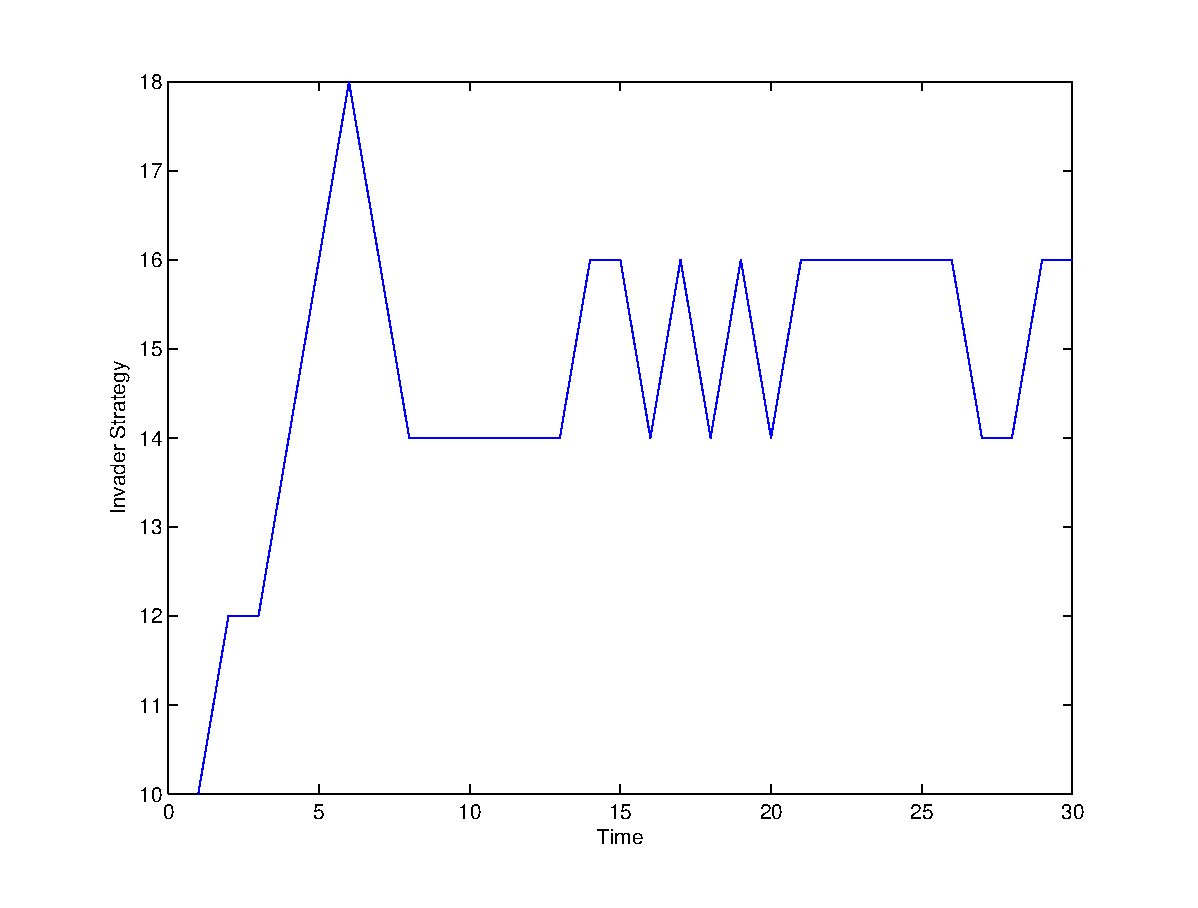
\includegraphics[width=\textwidth]{greedy_optimization_invader.eps}
%\end{center}
%\caption{The evolution of the invader's strategy over time: at first it increases and then oscillates between two high strategies.}
%\end{subfigure}
\begin{subfigure}{.5 \textwidth}
\begin{center}
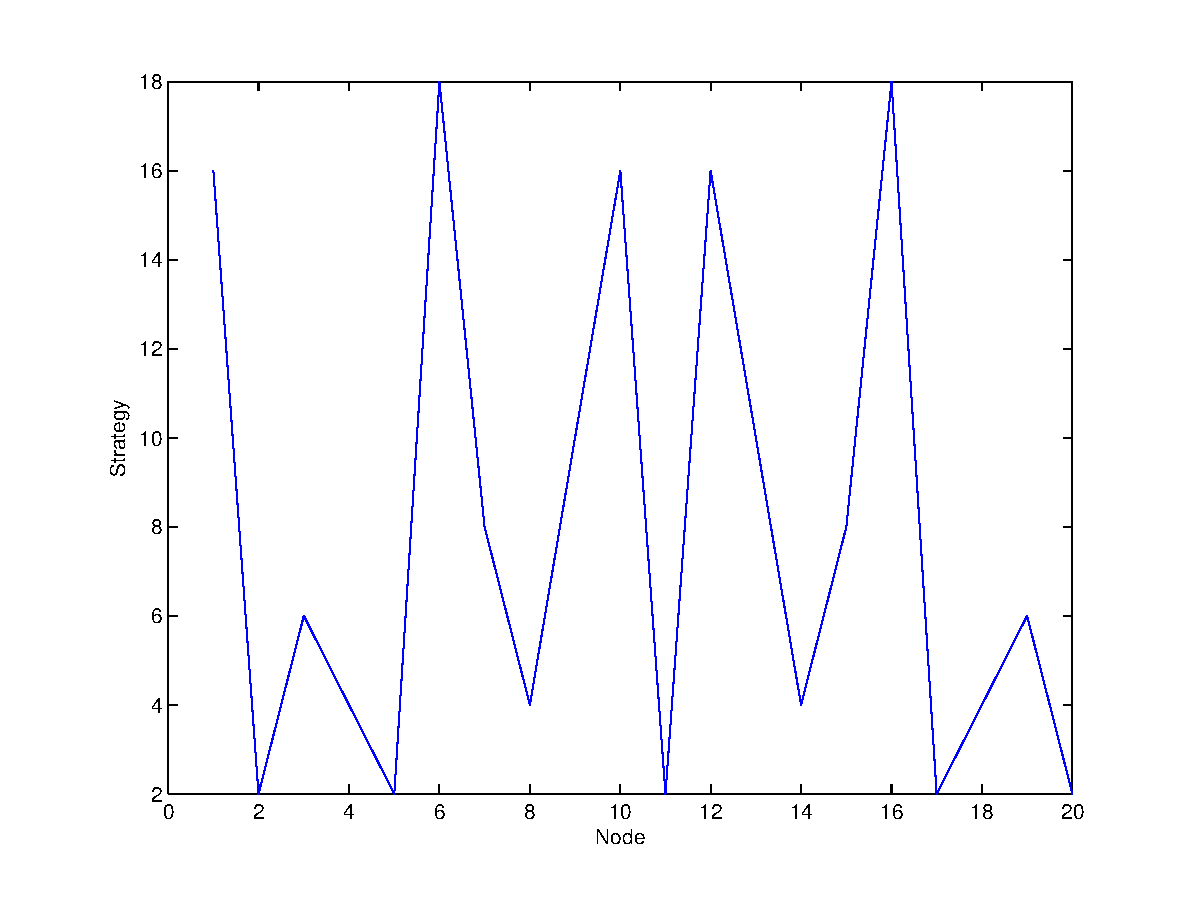
\includegraphics[width=\textwidth]{end_of_greedy_optimization.eps}
\end{center}
\caption{The end result of a greedy optimization, where the $x$-axis represents the nodes and the $y$-axis the final strategy.  The node that started with a different strategy, $10$ as opposed to $2$ is first.  The greedy optimization results in spatial periodicity in strategy.}
\end{subfigure}
\begin{subfigure}{.5 \textwidth}
\begin{center}
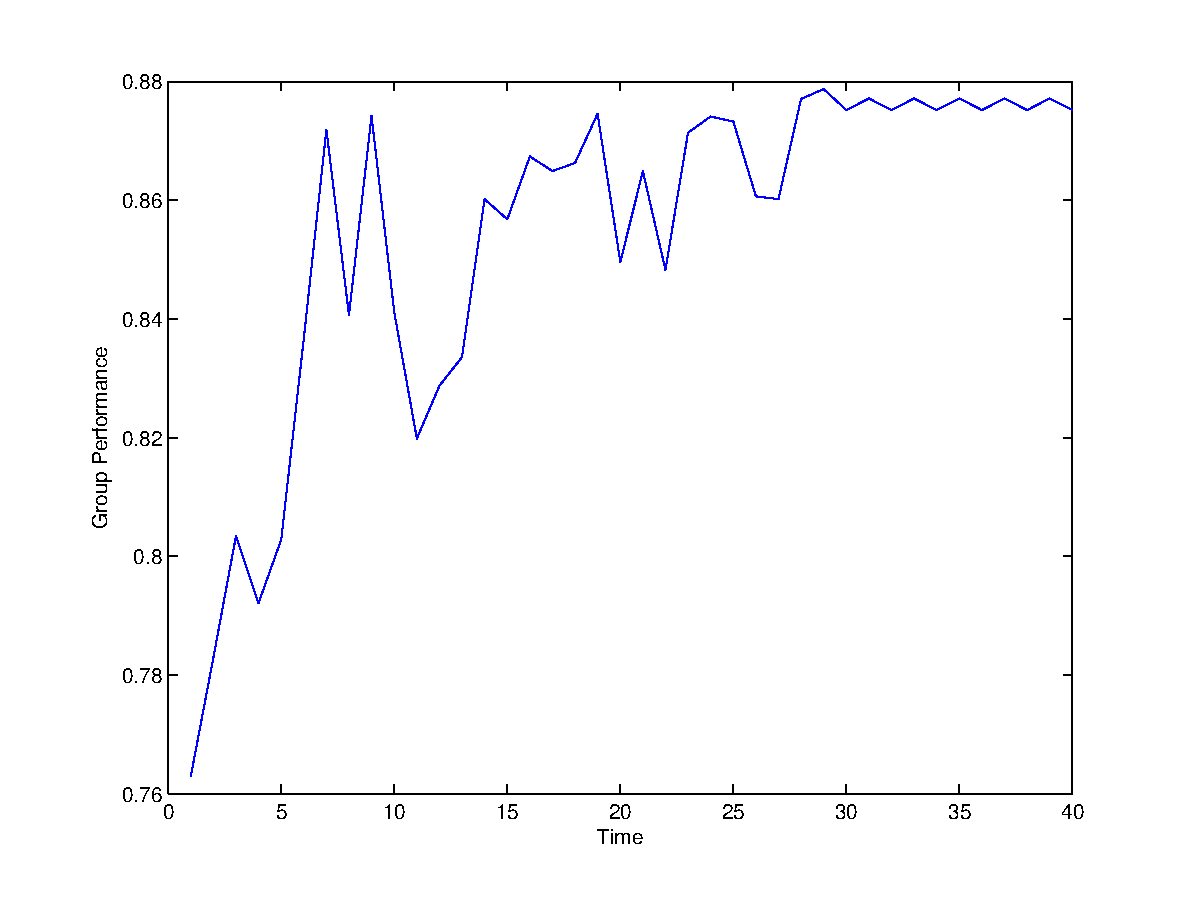
\includegraphics[width=\textwidth]{greedy_optimization_group_perf.eps}
\end{center}
\caption{Group performance changes over time as the nodes perform the greedy optimization.  The greedy optimization tends to increase overall group performance.}
\end{subfigure}
\caption{\label{greedy_opt} The results of a greedy optimization, where at each time step each node increases its strategy by $2$, decreases its strategy by $2$, or stays the same, depending on which performs best given that the rest of the network has the strategies they do.  Initially, the population all has strategy $2$, except for the first node which has strategy $10$. ($\alpha=.5,$ $N=20$)}
\end{figure}

%\begin{figure}
%\begin{subfigure}{.5 \textwidth}
%\begin{center}
%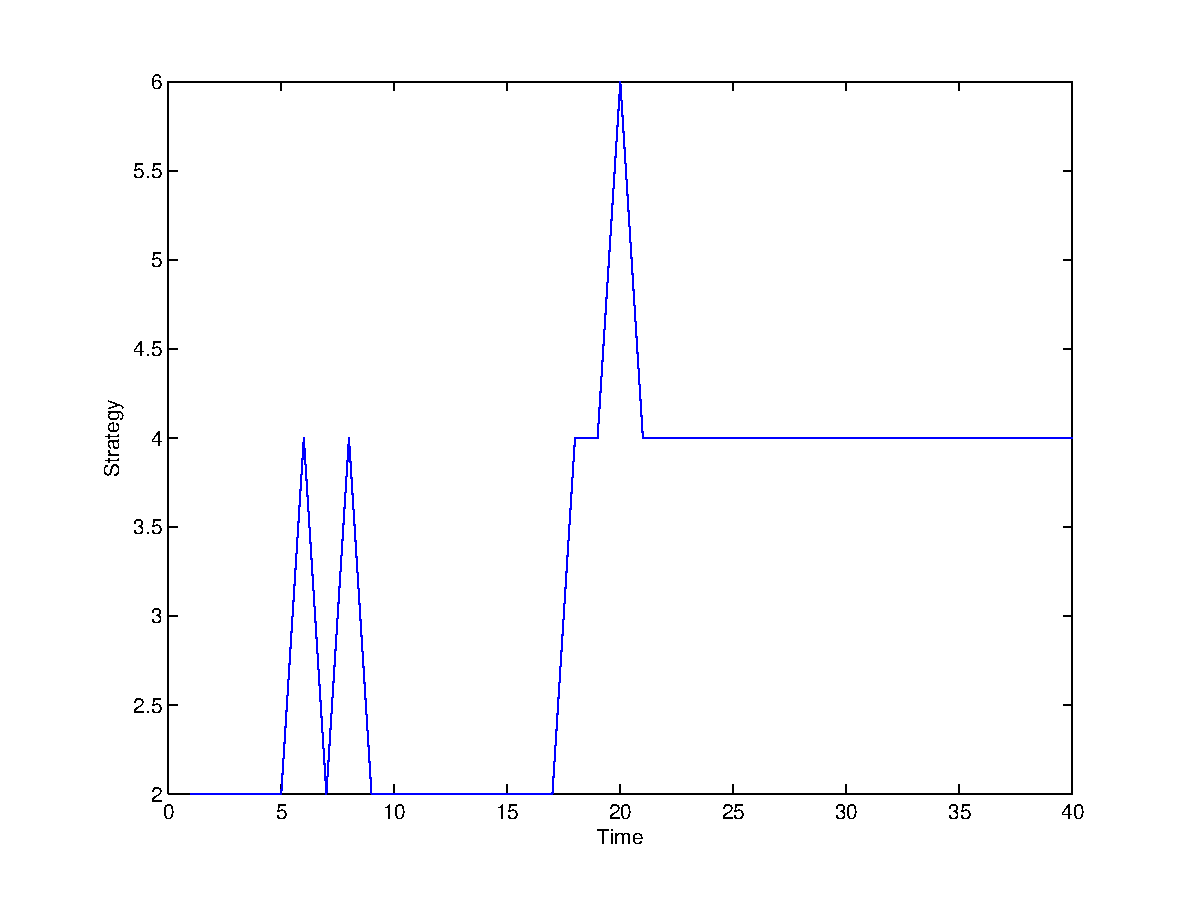
\includegraphics[width=\textwidth]{greedy_optimization_invader_v2.eps}
%\end{center}
%\caption{The evolution of the invader's strategy over time: at first it increases and then oscillates between two high strategies.}
%\end{subfigure}
%\begin{subfigure}{.5 \textwidth}
%\begin{center}
%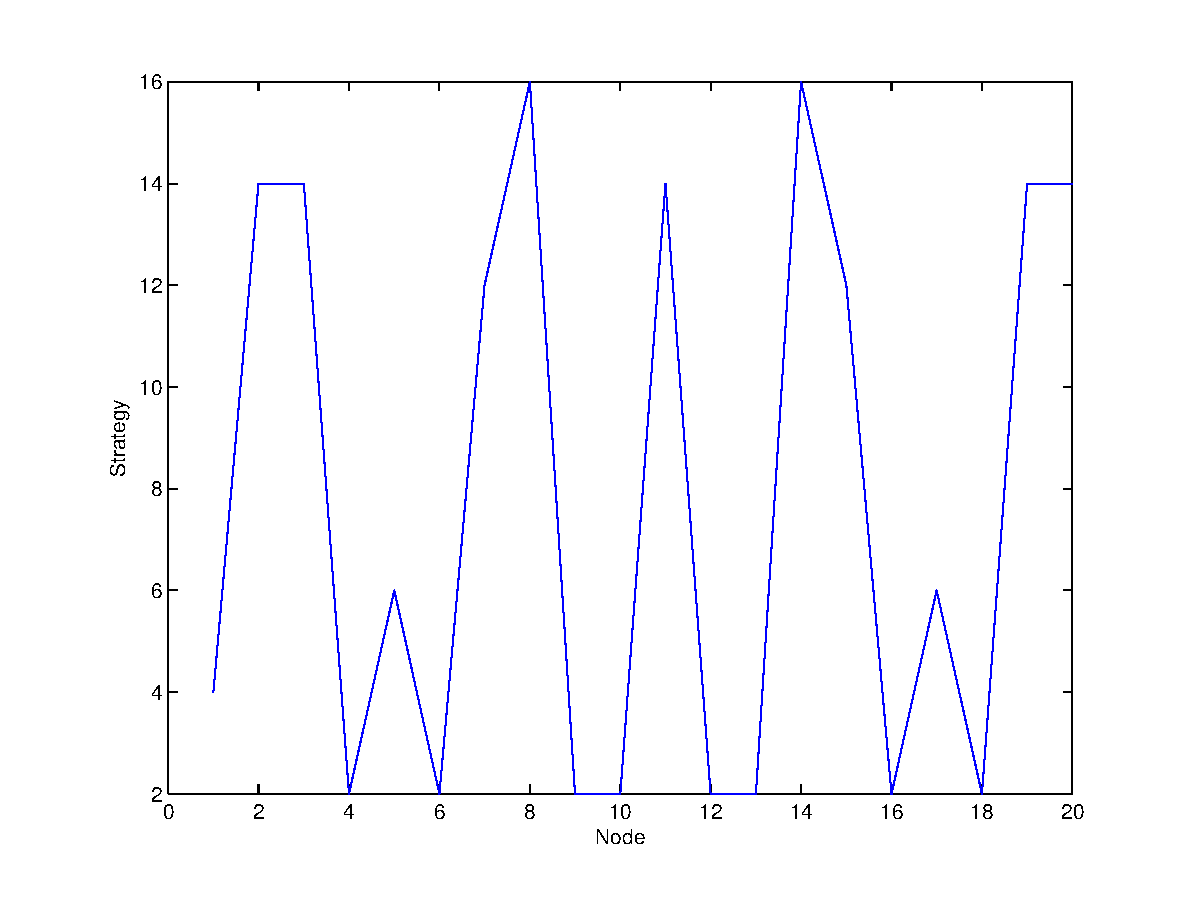
\includegraphics[width=\textwidth]{end_of_greedy_optimization_v2.eps}
%\end{center}
%\caption{The end result of a greedy optimization, where the $x$-axis represents the nodes and the $y$-axis the final strategy.  The node that started with a different strategy, $10$ as opposed to $2$ is first.  The greedy optimization results in spatial periodicity in strategy.}
%\end{subfigure}
%\begin{subfigure}{.5 \textwidth}
%\begin{center}
%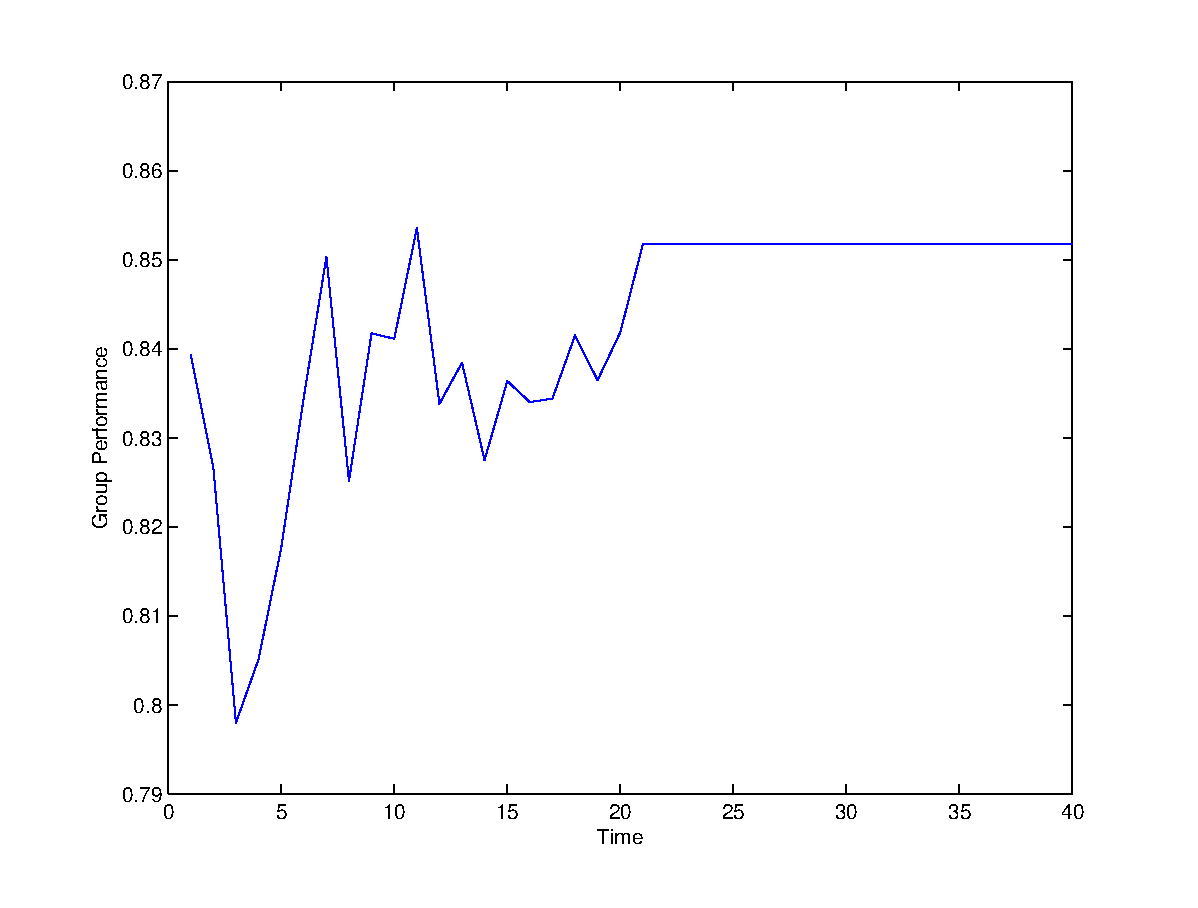
\includegraphics[width=\textwidth]{greedy_optimization_group_perf_v2.eps}
%\end{center}
%\caption{Group performance changes over time as the nodes perform the greedy optimization.  There is a large drop immediately and little subsequent change.}
%\end{subfigure}
%\caption{\label{greedy_opt_v2} The results of a greedy optimization, where at each time step each node increases its strategy by $2$, decreases its strategy by $2$, or stays the same, depending on which performs best given that the rest of the network has the strategies they do.  Initially, the population all has strategy $10$, except for the first node which has strategy $2$. ($\alpha=.5,$ $N=20$)}
%\end{figure}

\begin{figure}
\begin{subfigure}{.5 \textwidth}
\begin{center}
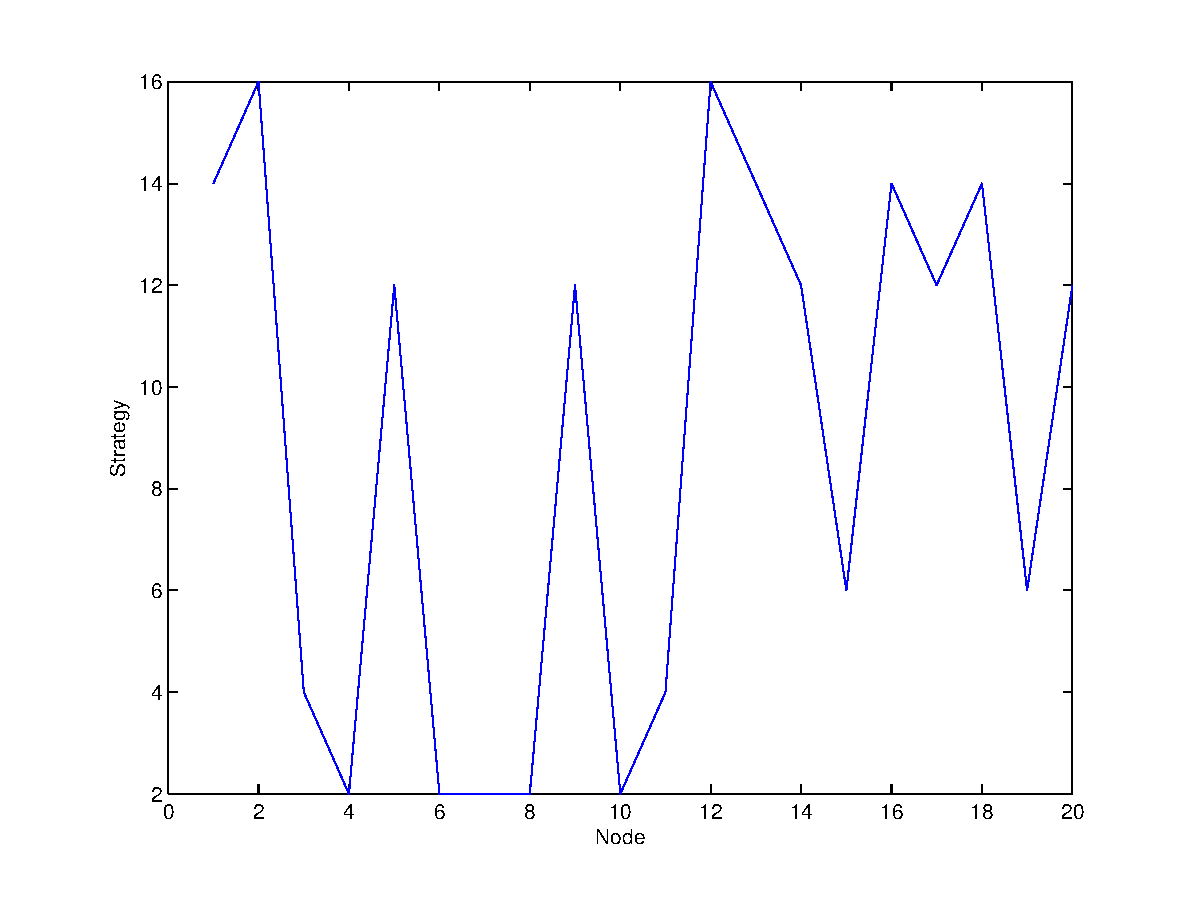
\includegraphics[width=\textwidth]{end_of_greedy_optimization_v3.eps}
\end{center}
\caption{The end result of a greedy optimization, where the $x$-axis represents the nodes and the $y$-axis the final strategy.  The node that started with a different strategy, $10$ in a population of $2$, is first.  The greedy optimization results in spatial periodicity in strategy.}
\end{subfigure}
\begin{subfigure}{.5 \textwidth}
\begin{center}
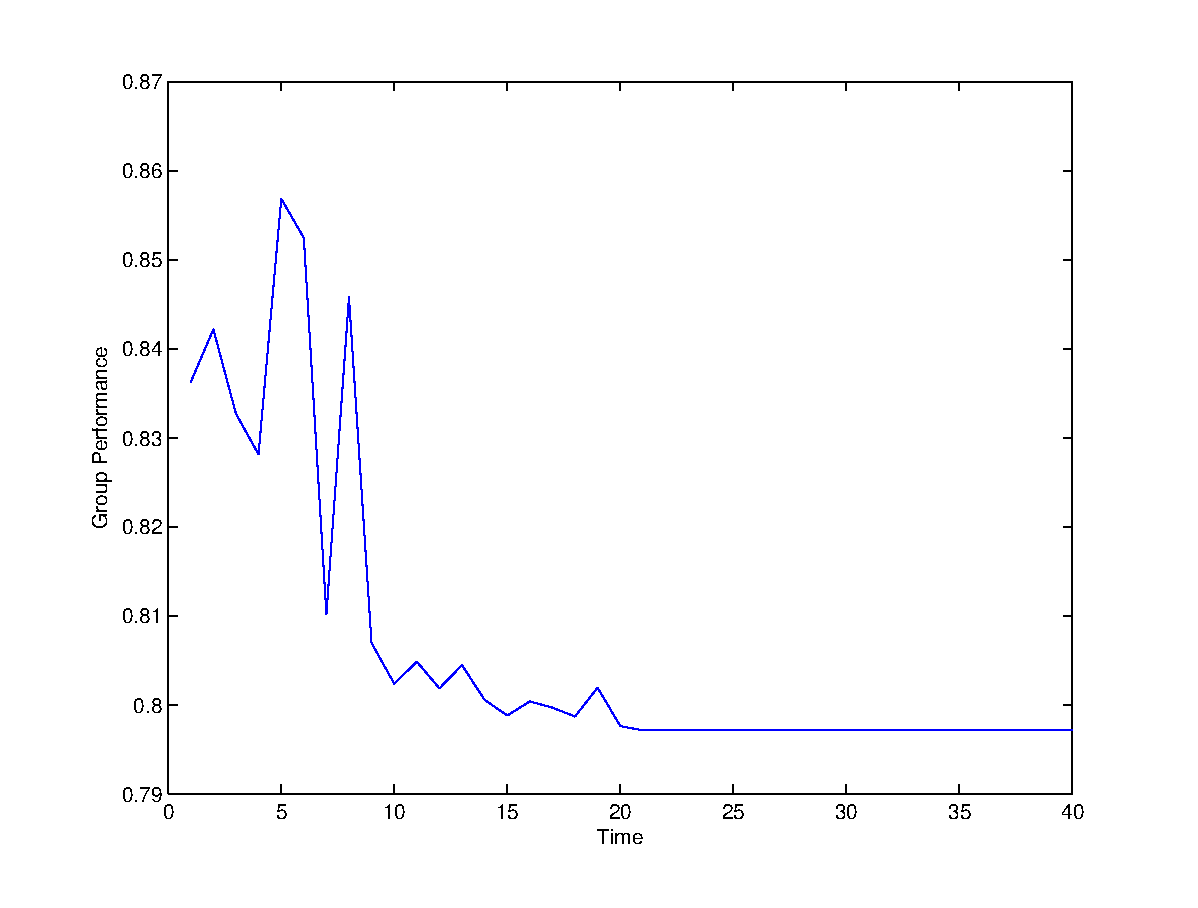
\includegraphics[width=\textwidth]{greedy_optimization_group_perf_v3.eps}
\end{center}
\caption{Group performance changes over time as the nodes perform the greedy optimization.  In this case, greedy optimization tends to decrease group performance.}
\end{subfigure}
\caption{\label{greedy_opt_v2} The results of a greedy optimization, where at each time step each node increases its strategy by $2$, decreases its strategy by $2$, or stays the same, depending on which performs best given that the rest of the network has the strategies they do.  Initially, the population randomly drawn strategies. ($\alpha=.5,$ $N=20$)}
\end{figure}



\section{Future Work}

\begin{enumerate}
\item prove Claim \ref{myconjecture} about eigenvalues
\item find ESS and CIS 
\item dependence of equilibria on the size of the network
\item Information centrality predicts the accuracy of each individual's opinion and eigenvector centrality predicts the speed of each individual's opinion.  Is there a measure that predicts performance when both speed and accuracy are valued?
\item prove that spatial periodicity in strategy is optimal for group performance
\item perform these analysis on more (empirical) networks
\end{enumerate}

\section{Conclusions }

\begin{enumerate}
\item from the perspective of network design, measure X tells how to optimize individual performance
\item optimal topology for the group when we also consider speed to consensus
\item group performance does or doesn't or in certain conditions (i.e. size of group, tradeoff between speed and accuracy) emerge out of individual level considerations so group performance does or doesn't or in certain conditions have to be invoked
\end{enumerate}

\nocite{*}
\bibliographystyle{plain}
\bibliography{info_evo}

\end{document}


